
\section{ModBB - Broad-band (pulse) propagation from Normal Modes}

{\bf ModBB} is designed to propagate the infrasonic signal produced by a transient source. {\bf ModBB} produces a broad band signal by Fourier synthesis of frequency-domain solutions obtained with either {\bf Modess} or {\bf WMod}. Modeling with {\bf ModBB} is thus restricted to propagation in a stratified atmosphere. {\bf CModess} has not been included because of the inordinately long runtimes that would be required as well as the severe restriction on frequency required to ensure convergence. 

To simulate broad band propagation using a normal mode model it is sufficient to compute the modal dispersion curves $\kappa_j(\omega)=k_j(\omega)+i\alpha(\omega)$ and mode functions $\psi_j(z,\omega)$ over a frequency band large enough to capture the spectrum of the signal source. Here $\omega=2\pi f$ is the angular frequency and $f$ is the cyclical frequency. {\bf ModBB} computes the dispersion curves and mode functions and saves them in files. Currently, the mode functions are computed and saved at a single altitude. Given a source spectrum or waveform, these files are then used as input to {\bf ModBB} for the synthesis of the resulting propagated waveform. {\bf ModBB} provides a model waveform which can be used to simulate the bandpassed signal from an explosive source. Arbitrary source waveforms or spectra can also be introduced through user-provided files. In addition, the bandpassed impulse response function can be computed. 

\subsection{Mathematical Background}
\label{sec: modbb math}

Let $P(r,z,t)$ be the deviation from mean pressure and use the notation introduced in section~\ref{sec: modess math}. Then {\bf ModBB} solves the generalized wave equation 
\begin{equation}
\left[  
\nabla_{H}^2 + \rho_0 \frac{\partial}{\partial z} \left ( \frac{1}{\rho_0} \frac{\partial}{\partial z} \right ) -\frac{1}{c^2} (\frac{\partial }{\partial t} + \textbf{v}_{0,H} \cdot \nabla_{H})^2 
\right] P(r,z,t) = 0 
\label{eq: wave_eqn}
\end{equation}
subject to the boundary condition 
\[
\frac {\partial P}{\partial z}\Big |_{z=0}= 0
\]
on the ground surface. If $s(t)$ is the pressure deviation extrapolated to $r=1\ \text{meter}$ and if 
\[
q(\omega)=\frac{1}{\sqrt{2\pi}}\int_{-\infty}^{\infty}s(t)e^{i\omega t} dt 
\]
are the Fourier components of $s$ then $P$ can be obtained by Fourier synthesis from a modal sum, $p$, as given by equation~\ref{eq: modess far field pressure}. For purposes of modeling the signal propagation by the linear propagation models considered here, $s(t)$ can be considered to be the waveform of the effective acoustic source signal. Using the fact that $P$ and $s$ are both real valued and changing integration variable from angular frequency $\omega$ to cyclical frequency $f$ one has 
\[
P(r,z,t) = \frac{1}{\sqrt{2\pi}}\int_{-\infty}^{\infty} q(\omega)p(r,z,\omega)e^{-i\omega t} d\omega 
= \text{Re}\sqrt{8\pi}\int_{0}^{\infty} q(2\pi f)p(r,z,2\pi f)e^{-2\pi ift} df .
\]


The motivation behind the design of {\bf ModBB} is to model the propagation of signals from large explosions. Such signals have abrupt onsets in the near field but decrease rapidly with time and can be said to be of finite duration. The nearly discontinuous signal onsets, however, lead to Fourier transforms which decrease slowly with increasing frequency and which generally cannot be well approximated by signals with finite bandwidth. Despite this the effective acoustic source signal can be modelled by a waveform with finite bandwidth. This is because of the atmospheric attenuation which increases rapidly with increasing frequency so that the high frequency components of the source signal do not propagate to the far field. 

Let the bandwidth of the effective source signal be less that $F$. Then the Fourier integral can be estimated by replacing the continuous integral by a finite discrete sum. Let the onset of the propagated signal occur after a time $T_0$ and let the duration of the signal be less than $T$ chosen so that the entire signal is contained in the interval between time $T_0$ and $T_0+T$. If the sum is produced by sampling evenly in frequency with sample spacing $\Delta f=\frac{1}{T}$ then the integral above can be efficiently estimated using the Fast Fourier Transform algorithm (FFT) (see, for example, \cite{Press:2007:NRE:1403886}). The FFT algorithm produces $P(r,z,t)$ sampled discretely in time with sample spacing $\Delta t=\frac{1}{F}$. The number of points summed over in the FFT is $N=TF$. Recall that, given the setup here, the FFT algorithm applied to a function of $t$ produces a periodic function $f$ with periodicity $F$ and the inverse transform produces a periodic function of $t$ with period $T$. Further, for the Fourier transform so obtained the positive frequency components are contained in the first $N/2$ points and the negative frequency components in the rest. Thus, for $m=0,1,2,\dots,N$, 
\[
P(r,z,T_0+m\Delta t) 
\approx 
\text{Re}\,\sqrt{8\pi}\Delta f \sum_{n=1}^{N/2-1} q(2\pi n\Delta f)p(r,z,2\pi n\Delta f)e^{-2\pi in\Delta fT_0}e^{-2\pi i\frac{nm}{N}}.
\]
Substituting from equation~\ref{eq: modess far field pressure} one obtains the formula that {\bf ModBB} computes: 
\begin{align}
P(r,z,T_0+m\Delta t) 
\approx 
\text{Re}\,\frac{i e^{-i \pi /4}}{\sqrt{r}} \sqrt{\frac {\rho_0(z)} {\rho_0(z_s)}} 
\Delta f \sum_{n=1}^{N/2-1} q(2\pi n\Delta f)&
\nonumber\\
\Big(\sum_j\psi_j(z_s,2\pi n\Delta f)\psi_j(z,2\pi n\Delta f) &
\frac{e^{i \kappa_j(2\pi n\Delta f)r}}{\sqrt{k_j(2\pi n\Delta f)}}\Big)
\nonumber\\&
e^{-2\pi in\Delta fT_0}e^{-2\pi i\frac{nm}{N}}.
\label{eq: modbb fft approx}
\end{align}
Since there are no modes at zero frequency the $n=0$ term is absent from the above sum. 

Note that once the modal wave numbers (modal dispersion curves) and mode functions are computed over the required range of frequencies equation~\ref{eq: modbb fft approx} can be evaluated. Recall from section\ref{sec: modess math} that in equation~\ref{eq: modbb fft approx} the range of wave numbers to be included in the modal sum must be determined prior to their being computed. The upper limit for the wave numbers is determined by the program itself. The lower limit is set by the user with the choice of maximum altitude of the computational domain. 

It is critical that the signal onset time $T_0$ and duration $T$ be chosen correctly. If parts of the signal are not contained in the interval between $T_0$ and $T$ then, due to the periodicity of discrete Fourier transforms, these parts will be aliased into the interval, overlapping with other parts of the waveform. Further, the truncation of the modal sum at a maximal phase velocity introduces a wave number cutoff which produces spurious arrivals. $T$ must be large enough to temporally separate these unphysical components of the output from the true waveform synthesis. 

\subsection{Running ModBB}
\label{sec:running modbb}

To model the propagation of a pulse two largely independent steps are required. First the modal wave number dispersion curves and mode functions must be computed. Then the computed values can be used to perform the modal sums and Fourier synthesis of equation~\ref{eq: modbb fft approx} for specified values of $r$. {\bf ModBB} is designed to perform these steps separately. First the dispersion curves and mode functions are computed using either {\bf Modess} or {\bf WMod} and saved to a file, called a dispersion file. Although the full mode functions are computed by both {\bf Modess} and {\bf WMod}, the current version of {\bf ModBB} only saves the mode functions at a given, fixed height. Once a dispersion file has been written and saved it can be used as input to a pulse propagation routine which evaluates equation~\ref{eq: modbb fft approx}. Producing a dispersion file is computationally expensive and can take some time. Once a dispersion file is written and saved computing a propagated waveform is essentially instantaneous. 

Signal duration and bandwidth are set during the computation of the dispersion curves. {\bf ModBB} requires the user to input the frequency step $\Delta f$ and bandwidth $F$ through options \verb+--f_step <df>+ and \verb+--fmax <F>+ respectively. Here \verb+<df>+ is the numerical value for $\Delta f$ and \verb+<F>+ the value for $F$. Once $\Delta f$ is set signal duration is also set through the relation $T=\frac{1}{\Delta f}$. $\Delta f$ and $F$ are the parameters with the greatest impact on runtimes. The number of modes increases quadratically with frequency so that as $F$ increases runtimes increase dramatically. Since $\frac{F}{\Delta f}$ is the number of individual frequencies required, the smaller $\Delta f$ is the more computations are required. On the other hand, it is not possible to simply reduce $T$ and $F$. $T$ must be larger than the duration of the propagated signal, typically $T$ can be on the order of 1000 seconds or for which $\Delta f$ is of the order of $0.001$ or less. $F$ must be large enough so that the effective source signal retains the characteristics of a signal from an explosive source: sudden positive pressure onset, one zero crossing, and a long negative pressure tail. We recommend that $F$ be chosen five times larger than the maximum frequency of the source signal under consideration. 

\begin{figure}
\begin{center}
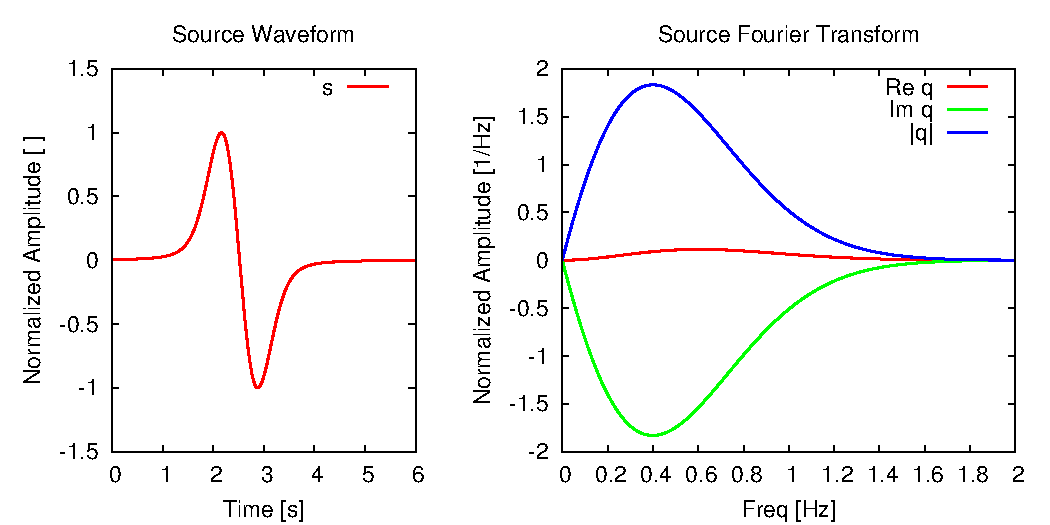
\includegraphics[scale=0.65]{figs/initial_pulse_model.pdf}
\end{center}
\caption{The built-in initial pulse with maximum Fourier transform frequency of 0.4 Hz and maximum frequency of 2 Hz. The waveform is shown in the left panel and the Fourier transform; real part, imaginary part, and magnitude; in the right panel. }
\label{fig: initial_pulse}
\end{figure}

For propagating a pulse a dispersion file is required as input. {\bf ModBB} provides four ways to input the effective acoustic source signal $s(t)$, either directly or through its Fourier transform $q(\omega)$. {\bf ModBB} can produce the band pass filtered impulse response function by setting $q=1$. This is equivalent to choosing $s(t)$ to be a delta function at $t=0$. Filtering, equivalent to a boxcar filter on the interval $-F<f<F$, is accomplished by the frequency bound in the dispersion file. {\bf ModBB} also has a built-in effective acoustic source function. The built-in source function has one adjustable parameter: the frequency of its maximum Fourier transform. Its waveform is normalized to have maximum amplitude of 1. The built-in source function with the maximum of its Fourier transform at 0.4 Hz is plotted in Figure \ref{fig: initial_pulse}. Both source waveform $s(t)$ and Fourier transform $q(\omega)$ are written to files \verb+source_waveform_input_example.dat+ and \verb+source_spectrum_input_example.dat+ each time the pulse propagation routines are run. These files have the format \begin{center}\verb+time[s] pressure[Pa]+\end{center} 
and 
\begin{center}\verb+freq[Hz] Re(Fourier transform)[Pa/Hz] Im(Fourier transform)[Pa/Hz]+\end{center} 
respectively. Finally, the input of user-provided source files is supported. The user can provide either a waveform file or a Fourier transform file, in the format given above for the built in source files. 


To run {\bf ModBB} make sure its executable is in the system's path and enter 
\begin{verbatim} 
    ModBB [--option1 val1] [--option2 val2] [...] [--flag1] [...] 
\end{verbatim}
on a command line. Generally, options are followed by values, either numbers, strings or filenames. Flags are not. Entering \verb"ModBB --help" sends the following help page to the screen: 
\begin{verbatim}
One of two algorithms can be used to perform pulse propagation. The first is
based on the Effective Sound Speed Approximation (as in Modess), the second is
based on the the Wide_Angle High-Mach solution of the wave equation (as in
WMod). Modess is faster but is accurate for launch angles less than 30 degrees
and low wind speeds. WMod extends the validity to higher angles and high Mach
numbers, but is slower.
To propagate a pulse, two steps must be completed:
1. A dispersion file must be calculated using the option --dispersion .
2. Pulse propagation is calculated for a selected source type:
  --source impulse : Delta function
  --source pulse1 : Built-in pulse type 1
  --source pulse2 : Built-in pulse type 2
  --source spectrum --source_file <filename> : User-supplied spectrum file
  Format: Freq Re[ spec(f) ] Im[ spec(f) ]
  --source waveform --source_file <filename> : User-supplied waveform file
  Format: Time Amplitude

The options below can be specified in a colon-separated file "modbb.param" or at
the command line. Command-line options override file options.

Options Control:
  --help                 Prints help test
  --paramfile            Parameter file name [modbb.param]
  --printparams          Print parameter summary to screen

Modes of Operation:
  --dispersion           Calculate dispersion at multiple frequencies
    --method             Calculation method. Currently supported: { modess, wmod
                         } [required]
    --dispersion_file    File to write dispersion results to [required]
    --azimuth            Azimuth of propagation, in degrees CW from North
                         [0,360) [required]
    --f_min              Minimum frequency in Hz [required]
    --f_max              Maximum frequency in Hz [required]
    --f_step             Frequency interval in Hz [required]
    --atmosfile          Atmospheric profile filename [required]
    --maxheight_km       Maximum height of analysis in km [150.0]
    --zground_km         Ground height [take from Z0 parameter in atmosfile, or
                         0.0]
    --Nz_grid            Number of vertical grid points to use [20000]
    --sourceheight_km    Source height in km [0.0]
    --receiverheight_km  Receiver height in km [0.0]
    --maxrange_km        Maximum range in km to use for modeling [1000.0]
    --Nrng_steps         Number of range steps to use [1000]
    --ground_impedence_model
                         Impedence model to use. Currently only "rigid" is
                         supported. [rigid]
    --Lamb_wave_BC       Use admittance = -1/2*dln(rho)/dz
    --write_atm_profile  Output atmospheric profile to atm_profile.nm
    --use_attn_file      File name containing attenuation, to override default
                         Sutherland/Bass [n/a]. Columns are
                         Height(km) Attenuation(np/m)
    --use_zero_attenuation
                         Set attenuation to zero.
    --wvnum_filter       Use wavenumber filter by phase speed. Requires --c_min
                         and --c_max
      --c_min            Minimum phase speed to keep
      --c_max            Maximum phase speed to keep
  --propagation          Calculate propagated waveform using dispersion results
    --input_dispersion_file
                         File to read dispersion results from [required]
    --output_waveform_file
                         File to write resultant waveform to [required]
    --source             Source type. Options include:
                         {impulse,pulse1,pulse2,spectrum,waveform} [impulse]
      --source_file      File containing the source spectrum or waveform, if
                         applicable
      --f_center         Center frequency for pulse1 or pulse2 options. Must be
                         <= f_max/5 [f_max/5]
    --nfft               Number of FFT points [4*f_max/f_step]
    --max_celerity       Maximum celerity for calculation [340.0]
    --receiver           Receiver type {single,multiple} [single]
      --range_km         Propagation range in km for a single receiver
      --start_range_km   Starting propagation range in km for multiple receivers
      --end_range_km     Ending propagation range in km for multiple receivers
      --range_step_km    Propagation range step in km for multiple receivers



OUTPUT Files: Format description (column order):
  <dispersion file>        Contains one line per frequency with entries:
                           freq, (# of modes), rho(z_src),
                           followed for each mode 'i' by quadruples:
                           real(k(i)), imag(k(i)), Mode(i)(z_src), Mode(i)(z_rcv)
  <waveform file>          t  P  (single receiver)
                           r  t  P  (multiple receivers)
Examples (run from 'samples' directory):
    ../bin/ModBB --dispersion --dispersion_file myDispersionFile.dat \
         --atmosfile NCPA_canonical_profile_zuvwtdp.dat --azimuth 90 --f_min \
         0.001953125 --f_step 0.001953125 --f_max 0.5 --method modess
 --or--
    ../bin/ModBB --dispersion --dispersion_file myDispersionFile.dat \
         --atmosfile NCPA_canonical_profile_zuvwtdp.dat --azimuth 90 --f_min \
         0.001953125 --f_step 0.001953125 --f_max 0.5 --method wmod

 --then--
    ../bin/ModBB --propagation --input_dispersion_file myDispersionFile.dat \
         --range_km 240 --output_waveform_file mywavf.dat --receiver single \
         --source impulse

    ../bin/ModBB --propagation --input_dispersion_file myDispersionFile.dat \
         --output_waveform_file mywavf.dat --receiver multiple \
         --start_range_km 240 --end_range_km 300 --range_step_km 20 --source \
         waveform --source_file source_waveform_input_example.dat

\end{verbatim}

As discussed above, {\bf ModBB} has two distinct functionalities: dispersion curves and mode amplitudes can be computed and written to a dispersion file and existing dispersion files can be used as input to a Fourier synthesis of a propagated pulse. To compute and save dispersion files one uses the option \verb+--out_disp_src2rcv_file+ followed by the name of the file. Dispersion files are computed using either {\bf Modess} or {\bf WMod}, the choice being made with the options \verb+--use_modess+ or \verb+--use_wmod+. The dispersion file format is a sequence of lines, one per frequency, beginning with the frequency and then containing the number of modes, the mean density of the atmosphere at source and receiver and then a sequence of horizontal wave numbers and mode amplitudes at source and receiver as in
\begin{verbatim}
freq n_modes rho_src rho_rcv Re(k_m_pert) Im(k_m_pert) V_m(z_src) V_m(z_rcv)
\end{verbatim} 
for \verb+m+ ranging from 1 to \verb+n_modes+. Additional options specific to \verb+--out_disp_src2rcv_file+ are \verb+f_step+, \verb+f_max+, and \verb+f_min+. The options \verb+f_step+ and \verb+f_max+ have been described above. The option \verb+f_min+ sets the frequency at which the dispersion file begins; it defaults to \verb+f_step+. Generally, no significant reduction in run time is achieved by setting \verb+f_min+ $>$ \verb+f_step+ since there are very few modes when the frequency is small. Setting \verb+f_min+ can be useful if one needs to compute dispersion files in several steps, to be concatenated into a single file afterwards. 

If either source or reveiver is on the ground the minimum required phase speed is estimated using the WKB approximation (see Fig.\,\ref{fig:wvnums_modess}). The option \verb+--turnoff_WKB+ forces the dispersion file to be written using the minimum of the effective sound speed as the minimum modal phase speed, rather than using the WKB approximation to estimate the lowest relevant phase speed. The option \verb+--use_zero_attn+ sets the attenuation to zero. In the current release this is done by setting the imaginary part of the wave numbers to zero, rather than by setting the attenuation to zero prior to writing the dispersion file. Since the imaginary part of the wave number is extimated in first order perturbation theory in Modess and Wmod setting the imaginary part to zero is equivalent to having set the attenuation coefficient to zero. 

To perform a Fourier synthesis of a propagated pulse one sets either \verb+--pulse_prop_src2rcv+, to propagate to a single receiver location, or \verb+--pulse_prop_src2rcv_grid+, to propagate to an array of receiver locations, followed, in both cases, by the name of the appropriate dispersion file. For both options a source type must be set as described above. If the built-in pulse is to be used, by setting \verb+--use_builtin_pulse+, then the frequency of maximum Fourier component must be set using \verb+--f_center+; the default value is $F/5$. The user provides an output file using \verb+--waveform_out_file+ followed by the output filename. When using \verb+--pulse_prop_src2rcv+ the range at which the waveform is to be computed must be set using \verb+--range_R_km+. If \verb+--pulse_prop_src2rcv_grid+ is being used then the smallest range in the receiver array, \verb+--R_start_km+, the largest range, \verb+--R_end_km+, and the spacing between ranges, \verb+DR_km+, must all be set. Distances are in kilometers. Note that the altitudes for source and receiver are set in the dispersion file. In all cases {\bf ModBB} computes the propagated waveform in a moving window. The window length is $T/\Delta f$ where $\Delta f$ is the value for \verb+--f_step+ from the dispersion file. The start of the window is set using the option \verb+--max_celerity+ followed by a value $c$. If $R$ is the range at which the waveform is being computed then the window starts at $T_0=R/c$. Note that with \verb+--pulse_prop_src2rcv+ the output file format is time, waveform, Hilbert transformed waveform, with the time record beginning at $T_0$. With \verb+--pulse_prop_src2rcv_grid+ data is stored in blocks of constant range with the format range, time, waveform and with each time record beginning at 0. 

Finally, the option \verb+--nfft+ sets the size of the FFT to be used in the waveform synthesis. Generally, using the number of frequencies in the dispersion file results in a poorly sampled waveform. Increasing the number of points used by zero padding improves the quality of the resulting waveform plots. It is to be emphasized that no new information is introduced in this way. The synthesized waveform is simply being more finely sampled. 

\subsection{Running ModBB: examples}
\label{sec: modbb examples}

As an example consider the following (note that this example is different from the ones that are on the {\bf ModBB} help page). Here a dispersion file is written for eastward propagation in the NCPA toy atmosphere. The bandwidth is chosen to be small, $F=0.5$ Hz, so that the file computes fairly rapidly. $\Delta f$ is chosen to be 0.002 corresponding to a time window, $T$, of 500 seconds. Calculations are done using {\bf Modess}. 

\begin{verbatim} 
    ../bin/ModBB --dispersion --disperson-file myDispersionFile.dat \
                 --atmosfile NCPA_canonical_profile_zuvwtdp.dat \
                 --azimuth 90 --method modess \
                 --f_min 0.002 --f_step 0.002 --f_max 0.5
\end{verbatim}

The dispersion file created above, \verb+myDispersionFile.dat+, is then used to propagate the built-in pulse to 270 km. \verb+--f_center+ is not set so that the default $F/5$, in this case 0.1 Hz, is used. Note that \verb+--max_celerity+ is set at 320 m/s rather than the default value of 300 m/s for which the resulting time window is not optimal. The waveform and Fourier transform for the built-in pulse is plotted in Figure \ref{fig: modbb ex built-in pulse}. The propagated waveform is plotted in Figure \ref{fig: modbb ex prop to 270 km}. 

\begin{verbatim}
    ../bin/ModBB --propagation --input_dispersion_file myDispersionFile.dat \
                 --range_km 270 --output_waveform_file mywavf.dat \
                 --source pulse1 --max_celerity 320
\end{verbatim}

\begin{figure}
\begin{center}
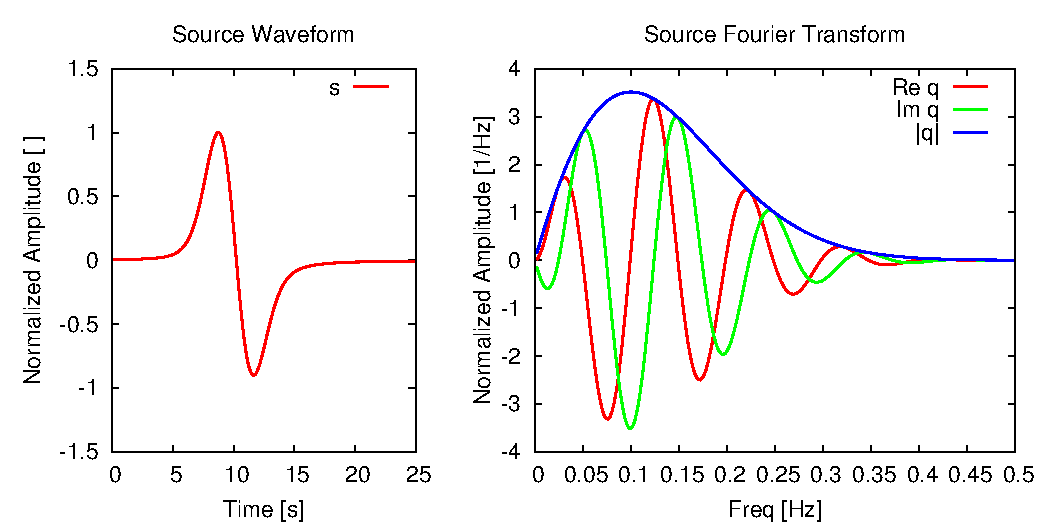
\includegraphics[scale=0.65]{figs/modbb_ex_source_model}
\end{center}
\caption{The built-in source waveform and Fourier transform with peak at 0.1 Hz.}
\label{fig: modbb ex built-in pulse}
\end{figure}

\begin{figure}
\begin{center}
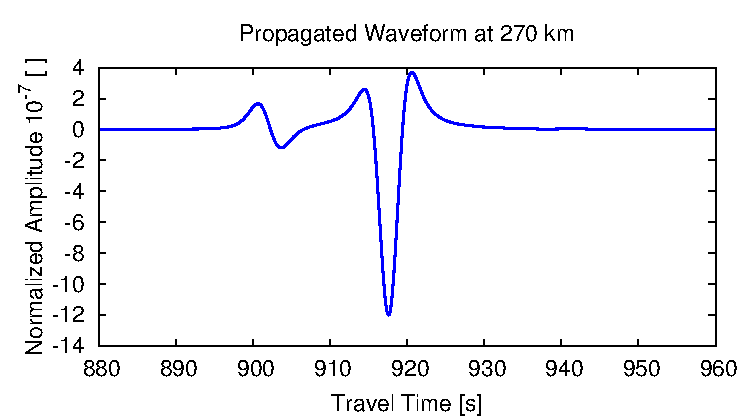
\includegraphics[scale=0.65]{figs/modbb_ex_prop_pulse}
\end{center}
\caption{Eastward propagation in the NCPA toy atmosphere. Propagated pulse to 270 km vs time.}
\label{fig: modbb ex prop to 270 km}
\end{figure}

The example below creates a grid of waveforms using \verb+--pulse_prop_src2rcv_grid+, propagating using the dispersion file created using the example above. Waveforms are written in 20 km increments starting at 220 km and ending at 300 km. Maximum celerity of 320 m/s was used rather than the default value. The results, shifted so that each time window begins at the appropriate $T_0$, are plotted in Figure \ref{fig: modbb ex prop 220 to 300 km}.

\begin{verbatim}
    ../bin/ModBB --propagation --input_dispersion_file myDispersionFile.dat \
                 --receiver multiple --output_waveform_file mywavf_grid.dat \
                 --start_range_km 220 --range_step_km 20 --end_range_km 300 \
                 --source pulse1 --max_celerity 320
\end{verbatim}

\begin{figure}
\begin{center}
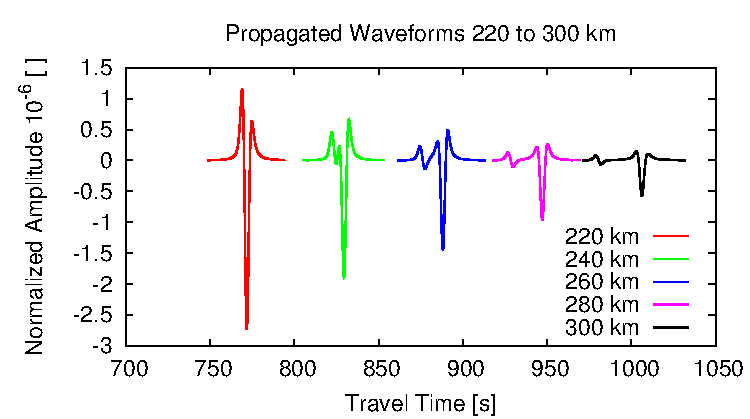
\includegraphics[scale=0.65]{figs/modbb_ex_prop_pulse_grid}
\end{center}
\caption{Eastward propagation in the NCPA toy atmosphere. Propagated pulse from 220 to 300 km vs time in increments of 20 km.}
\label{fig: modbb ex prop 220 to 300 km}
\end{figure}

